\chapter{Parte 1}
\label{ch:into} % This how you label a chapter and the key (e.g., ch:into) will be used to refer this chapter ``Introduction'' later in the report. 
% the key ``ch:into'' can be used with command \ref{ch:intor} to refere this Chapter.

La soluzione ad attori del problema degli Assignement precedenti è stata implementata in java, utilizzando la libreria Akka.

\section{Struttura del Sistema ad Attori e Descrizione Operativa}

La gerarchia è composta da tre principali livelli di attori: \textbf{Boss}, \textbf{Pm} e \textbf{Employee}, ciascuno con ruoli e responsabilità ben definiti.

\subsection{Livello 1: Boss}
L'attore \textbf{Boss} è la radice della gerarchia ed è responsabile dell'intero processo di gestione dei task. Riceve il percorso di una directory (\texttt{directoryPath}) e popola una lista di compiti (\texttt{pathList}) utilizzando la funzione \texttt{Utils.populateListOfPaths}. Dopo aver suddiviso i compiti in sottogruppi basandosi sul numero di lavoratori disponibili, il \textbf{Boss} invia un messaggio \texttt{Pm.Order} al suo subordinato \textbf{Pm}, specificando:
\begin{itemize}
    \item La directory di lavoro.
    \item I compiti da eseguire suddivisi in blocchi.
    \item Eventuali riferimenti per risposte future.
\end{itemize}

Inoltre, il \textbf{Boss} monitora l'elaborazione tramite i report inviati dagli \textbf{Employee}, aggiornando i dati attraverso un’interfaccia che organizza i risultati dei task. Questo lo rende il punto centrale della raccolta dei risultati.

\subsection{Livello 2: Pm (Project Manager)}
Il \textbf{Pm} agisce come intermediario tra il \textbf{Boss} e i lavoratori effettivi (\textbf{Employee}). Al momento della creazione, genera una serie di attori \textbf{Employee}, il cui numero è specificato dalla costante \texttt{NUMBER\_OF\_WORKERS}. Il \textbf{Pm} riceve i compiti dal \textbf{Boss} e li assegna ai suoi lavoratori utilizzando il messaggio \texttt{Ordered}, suddividendo equamente i task.  

Durante l'elaborazione, il \textbf{Pm} riceve i report dagli \textbf{Employee} tramite messaggi di tipo \texttt{Employee.Report} e li inoltra al \textbf{Boss}.  

In caso di comandi globali come la pausa (\texttt{StopMsg}) o la ripresa (\texttt{ResumeMsg}), il \textbf{Pm} inoltra i messaggi a tutti gli \textbf{Employee}, garantendo un controllo centralizzato.

\subsection{Livello 3: Employee}
Gli attori \textbf{Employee} rappresentano i lavoratori del sistema. Ognuno riceve un insieme di compiti dal \textbf{Pm} e li elabora uno alla volta. Le principali caratteristiche di un \textbf{Employee} includono:
\begin{itemize}
    \item \textbf{Gestione Asincrona dei Task:} I task vengono elaborati utilizzando una funzione di utilità (\texttt{Utils.linesWithBufferInputStream}) e i risultati vengono inviati tramite un report al mittente (di norma il \textbf{Pm}).
    \item \textbf{Pausa e Ripresa:} Gli \textbf{Employee} possono fermare l'elaborazione dei task tramite il messaggio \texttt{StopMsg} e riprenderla tramite \texttt{ResumeMsg}. Questa capacità migliora la resilienza del sistema e consente una gestione flessibile dei lavoratori.
    \item \textbf{Chiusura Ciclica dei Task:} Utilizzano un iteratore (\texttt{taskIterator}) per avanzare nel ciclo di compiti assegnati e inviano notifiche al completamento.
\end{itemize}

\subsection{Interazione tra gli Attori}
L'interazione tra gli attori è basata su un flusso di messaggi ben definito:
\begin{enumerate}
    \item \textbf{Boss → Pm:} Invio dei compiti tramite \texttt{Pm.Order}.
    \item \textbf{Pm → Employee:} Assegnazione dei task tramite \texttt{Ordered}.
    \item \textbf{Employee → Pm:} Invio dei risultati dei task tramite \texttt{Employee.Report}.
    \item \textbf{Pm → Boss:} Trasmissione dei report degli \textbf{Employee}.
\end{enumerate}

Questa struttura modulare rende il sistema scalabile e facile da mantenere, poiché ogni livello si occupa esclusivamente di un insieme ben definito di responsabilità.

% \subsection{Vantaggi del Design}
% \begin{enumerate}
%     \item \textbf{Modularità:} Ogni attore ha ruoli chiari, facilitando estensioni o modifiche.
%     \item \textbf{Parallelismo:} L'uso degli attori consente un'elaborazione parallela dei task.
%     \item \textbf{Resilienza:} La gestione di eventi come pause e riprese garantisce continuità operativa.
%     \item \textbf{Scalabilità:} È possibile aggiungere più attori \textbf{Pm} o \textbf{Employee} per gestire un numero maggiore di compiti senza modificare l'architettura principale.
% \end{enumerate}

\begin{figure}[h]

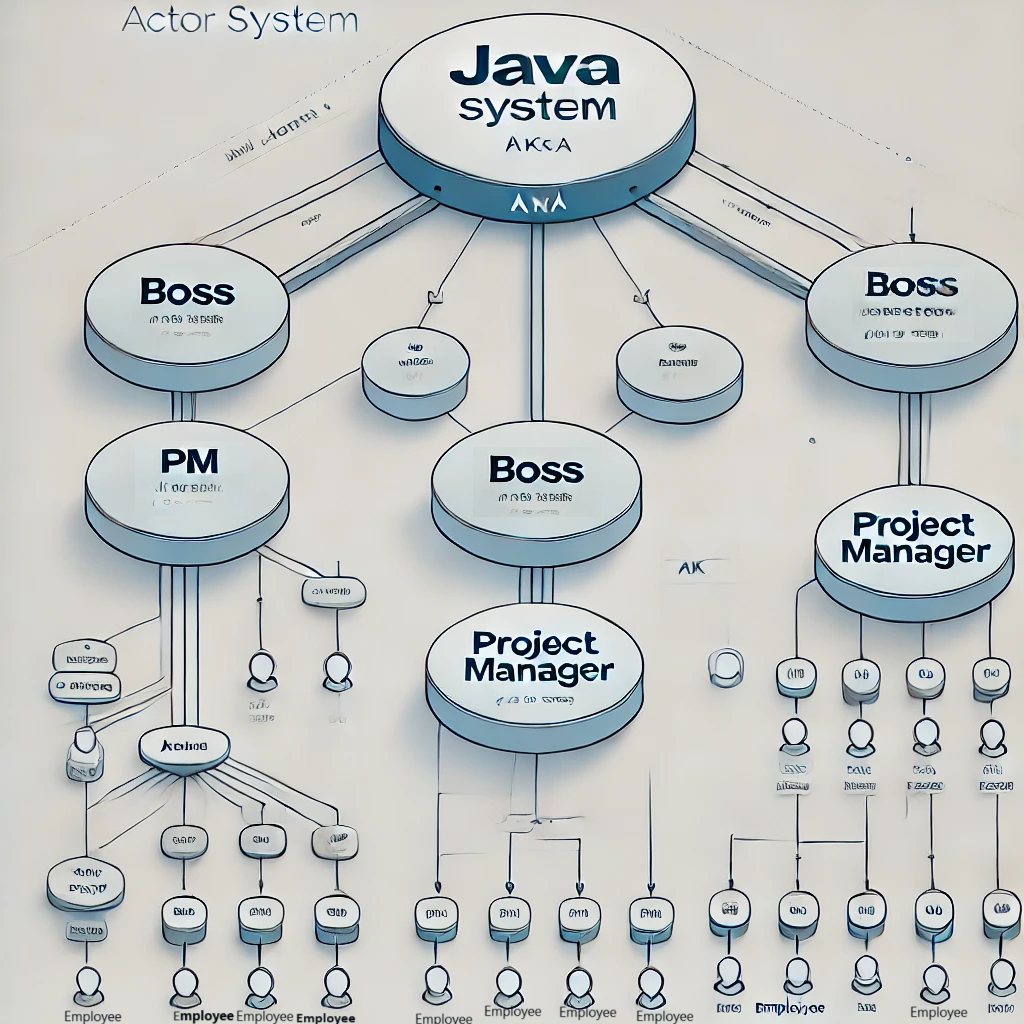
\includegraphics[width=15cm]{report/img/chaGpt-graph.png}\\[0.5cm]
\caption{Architettura del sistema (disegnata con chatgpt)}
\end{figure}
